% !TeX root = ../../main.tex
\chapter{Contribution}

In this chapter it is presented the conceptualization of a proposed Scala-based reference architecture for enabling the development of cross-platform, polyglot and distributed libraries and frameworks.

Its discussion is structured as follows.
%
First, the intents and application scenarios motivating the proposed architecture are discussed.
%
Subsequently, the corresponding requirements and constraints are formalized.
%
Thereafter, the elements composing the architecture are presented.
%
Finally, the implications of adopting this design are analyzed.

\section{Intents}

The intents of the proposed architecture are to enable the development of distributed Scala libraries and frameworks to be both cross-platform, that is, able to run on multiple platforms and runtimes; and polyglot, that is, designed to be able to interoperate with its public interface from multiple programming languages.
%
Both intents must be achieved while maintaining a unified and unique version of the components implementing the application logic of the software product.

\section{Application scenarios}

\section{Requirements}

Requirements describe formally the boundary of applicability of the proposed architecture and the conditions it is designed to satisfy.
%
These can be categorized into \textit{user}, \textit{system} and \textit{implementation} requirements and concern two types of users: \textit{end-users}, that are the developers intended to use the libraries and frameworks designed following the proposed architecture, henceforth simply \textit{library}; and \textit{developers}, that are the ones designing and implementing such libraries and frameworks.

\subsubsection{User requirements}

\begin{enumerate}[label=U\arabic*.]
    \item End-users interact with the library from multiple programming languages through a consistent API exploiting its functionalities while benefiting from language-specific ecosystem features. Supported languages include:
    \begin{itemize}
        \item Scala;
        \item Java;
        \item JavaScript; 
        \item TypeScript;
        \item C and C++.
    \end{itemize}
    \item End-users are able to write their own code leveraging the library functionalities:
    \begin{itemize}
        \item using Scala, with deployment possibly spanning across multiple platforms and runtimes:
        \begin{itemize}
            \item JVM;
            \item JavaScript environments, both in browser and server-side (Node.js);
            \item Native environments. These include desktop, server or System on Chip (SoC) devices running on 64-bit and ARM architectures.
        \end{itemize}
        \item using other supported languages (Java, JavaScript, TypeScript, C, C++), targeting their respective native platforms.
    \end{itemize}
    \item End-users are able to distribute the execution of their code leveraging the library functionalities across multiple machines exploiting some distributed communication mechanism, running on top of different platforms and runtimes, and possibly programmed in different languages.
\end{enumerate}

\todo{different environments because of different requirements}

\subsubsection{System requirements}

\begin{enumerate}[label=S\arabic*.]
    \item Library application logic is implemented once and reused across all supported platforms and runtimes. Modifications to the application logic must be applied only once and automatically reflected across all supported platforms and runtimes.
    \item Library API is consistent across all supported languages and it behaves uniformly regardless of the target platform, runtime or programming language.
\end{enumerate}

\subsubsection{Implementation requirements}

\begin{enumerate}[label=I\arabic*.]
    \item Developers implement the library using Scala, enabling them to harness functional programming, type-safe abstractions, expressive syntax and compositional design patterns to facilitate the development of robust, scalable, distributed, and concurrent software systems.
\end{enumerate}

\section{Constraints}

The proposed architecture imposes a fundamental constraint that significantly influences architectural decisions: all dependencies must support multi-platform compilation across target platforms. 
%
Where such multi-platform support is unavailable, platform-specific implementations must be provided to bridge the abstraction gap.
%
If an existing Scala library heavily relies on platform-specific dependency or its design is tightly coupled with a specific platform or runtime, adapting it to the proposed architecture may prove impractical or require substantial reengineering efforts.

For example, a distributed Scala library heavily relying on Akka and its actor model, together with its remoting and clustering capabilities, would require a complete redesign to be adapted to the proposed architecture, since Akka is JVM-only.
%
Moreover, when such platform-specific dependencies are essential for achieving critical non-functional requirements---such as fault tolerance or scalability attributes---that cannot be replicated though multi-platform alternatives, the adaptation becomes not merely impractical but potentially unfeasible.
%
In these cases, the tight coupling to a specific platform represents an architectural constraint rather than an implementation detail, and the proposed architecture may not constitute a suitable approach for such libraries without fundamentally revisiting their core design principles.

\section{Architectural elements}

The proposed architecture, presented in \Cref{fig:reference-architecture}, is composed by three main elements:

\begin{enumerate}
    \item a \textbf{pure core module}, implementing the application logic of the library. This module is designed to be platform-agnostic and independent of any specific technology or runtime;
    \item a \textbf{cross-platform infrastructure module}, responsible for enabling the distribution of the library functionalities across multiple end nodes and platforms and runtimes interaction. This includes a \textbf{general cross-platform and polyglot serialization binding}, providing the capability to marshal and unmarshal data structures exchanged between different platforms, runtimes and programming languages;
    \item a \textbf{polyglot library abstraction layer}, exposing a simplified and consistent interface API to end-users through different programming languages.
\end{enumerate}

1. and 2. are part of the so-called \textit{Software Product}, i.e. where the core functionalities of the library are implemented and the value is created.
%
3. is part of the \textit{User-to-Product Interface}, i.e. the interface through which end-users interact with the software product in their language of choice by accessing library functionalities through native packages generated by the polyglot library abstraction layer.

\begin{figure}
    \centering
    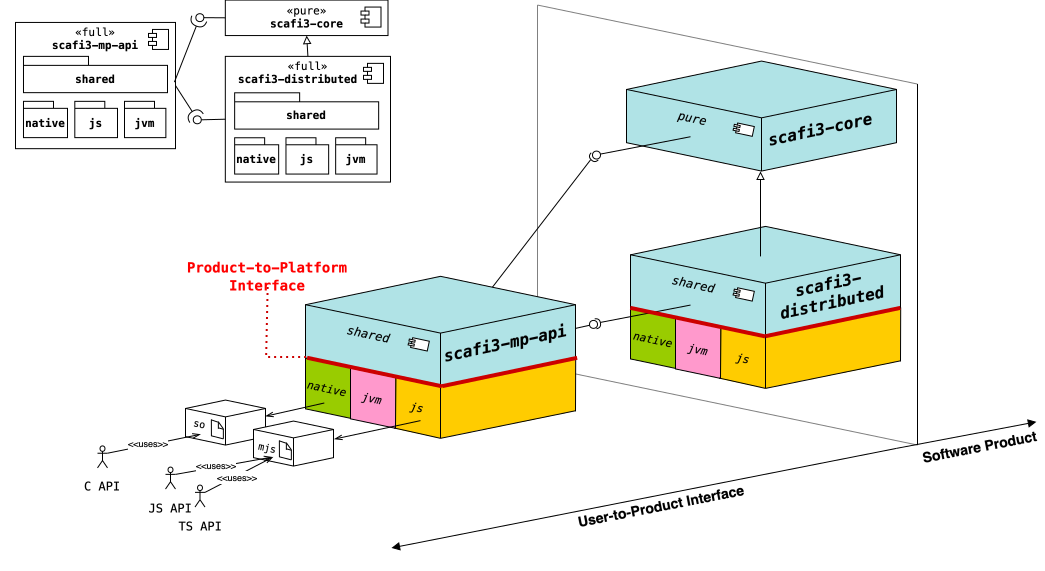
\includegraphics[width=\textwidth]{resources/img/architecture.pdf}
    \caption{Proposed reference architecture for cross-platform, polyglot and distributed Scala libraries and frameworks.}
    \label{fig:reference-architecture}
\end{figure}

\subsection{Pure library core module}

- designed to be platform- and technology-agnostic

- designed to be independent from distribution mechanism or any other infrastructural concern

- pure scala multiplaform

- exposes functionalities through well-defined interfaces

\subsection{Cross-platform distribution module}

- responsible for enabling distribution of library functionalities across multiple end nodes and platforms and runtimes interaction

- implement distribution mechanisms 

- can be implemented using adapters for different technologies, ref. to the clean architecture pattern

\subsection{Support for a general cross-platform and polyglot serialization binding}

- general serialization binding

- format agnostic and interoperable

\subsection{Polyglot library abstraction layer}

- exposes simplified and consistent interface API to end-users through different programming languages

- isomorphisms and portable types

\section{Consequences}

\begin{enumerate}
    \item The expressiveness of exchanged messages is limited to the capabilities of the serialization binding adopted.
\end{enumerate}
